\begin{document}
\title{COMS3008A Assignment -- Report}
\author{Sahil Dinanath, Darshan Singh}
\date{5 June 2023} 
\maketitle 
%\thispagestyle{empty}
\pagestyle{fancy}
\fancyhf{}
\fancyhead[R]{\thepage}
\fancyhead[L]{COMS3008A Assinment}
%\vskip 3mm 
%\pagenumbering{roman}
%\newpage
\pagenumbering{arabic} 
\section{Problem 1: Parallel Scan}
\begin{itemize}
	\item  Given a set of elements, $[a_0,a_1,\dotsm,a_{n-1}]$, the scan operation associated with addition operator for this input is the output set $[a_0,(a_0+a_1),\dotsm,(a_0+a_1+\dotsm+a_{n-1})]$. 
	\item For example, the input set is $[2,1,4,0,3,7,6,3]$, then the scan with addition operator of this input is $[2,3,7,7,10,17,23,26]$. 
\end{itemize}
\subsection*{Approach}
\subsection{Serial} 
\subsection*{strategy:}
The approach that was chosen to represent the serial implementation of the prefix scan algorithm was the serial workefficient implementation of blelloch's algorithm which is shown in Listing \ref{lst:scan_serial_blelloch}. 
\begin{lstlisting}[language=C, caption={upsweep and downsweep pseudocode}, label={lst:scan_serial_blelloch}]

upsweep(inputArray,n):
	for d = 0 to log2(n) - 1 do
    	for k = 0 to n - 1 by 2^(d+1) do
        	inputArray[k + 2^(d+1) - 1] += inputArray[k + 2^d - 1]


downsweep(inputArray,n):
	input[n-1] = 0
	for d = log2(n) - 1 down to 0 do 
		for k = 0 to n - 1 by 2^(d+1)do 
			temp = inputArray[k + 2^d - 1] 
			inputArray[k + 2^d - 1] = inputArray[k + 2^(d+1) - 1]
			inputArray[k + 2^(d+1) - 1] += temp

\end{lstlisting}
The idea as stated in \href{https://developer.nvidia.com/gpugems/gpugems3/part-vi-gpu-computing/chapter-39-parallel-prefix-sum-scan-cuda}{Parallel Prefix Sum with Cuda} is to build a balanced binary tree with n leaves and log2(n) levels

\subsection*{pseudocode:} 
\subsection{OpenMP}
\subsection*{parallization method:}
The serial implementation of blelloch's algorithm was used as the base for the OMP parallel implementation, with largely the core algorithm staying the same. However, the differences being with how the algorithm processed a single array. The first most obvious parallisation method is to parallise the inner for loops in both the upsweep and downsweep of the algorithm, see Listing \ref{lst:scan_parallisation_inner_loop} 
\begin{lstlisting}[language=C, caption={parallisation of the inner loop}, label={lst:scan_parallisation_inner_loop}]
...
		for k = 0 to n - 1 by 2^(d+1) in parallel do
...
\end{lstlisting}
this allows for the summations at each depth to be parallized. The issue with this method is that at each level the amount of elements that needs to be computed is halved, hence the algorithm becomes more serial as it progresses as there is less elements to split between the cores for both the up and down sweep.\\\\ The second parallization strategy was to take the input array, break it up into chunks and have each processor perform it's own up and down sweep on it's section of the array. This would expose more concurrency as at each depth all the processors can be acting on their chunk of the array, in contrast to the original method where at the highest depth only 1 processor will be able to act.\\This was achieved using a processor sum, which is the summation of each chunk given to each processor. Each processor then perform the up and down sweep on their respective chunk. Finally each processor adds their processor sum to each element of their array. 
eg: $[a_0,(a_0+a_1),(a_0+a_1+a_3),(a_0+a_1+a_3+a_4)]$\\
\\ assume 2 processors hence 2 chunks:\\
$[a_0,(a_0+a_1),(a_0+a_1+a_3)]$,\\$[(a_0+a_1+a_3+a_4),\dots]$\\
\\let $processorSum_0 = a_0+a_1+a_3$ therefore\\
$[(processorSum_0+a_4),(processorSum_0 + a_4 +a_5),\dots] $\\\\hence for each$ [(a_4),(a_4 +a_5),\dots]$ add $processorSum_0$\\
as you can see now each chunk is independant of eachother meaning we can now perform the up and down sweep independantly and concurrently on each processor. See Listing \ref{lst:scan_second_parallization_method} 
\begin{lstlisting}[language=C, caption={Serial Sequenctial Scan Algorithm with + operator}, label={lst:scan_second_parallization_method}]
getProcessSum(inputArray, size, processSum, chunkSize,rank){ 
	if (rank == 0):  
		processSum = 0 
		return 
	 
	start = (rank-1) * chunkSize 
	end = rank * chunkSize
	
	for i = start to end-1 by i+1 in parallel do
		processSum += input[i];
	 
applyOffset(inputArray, startIndex, endIndex, processSum,rank){ 
	sum = 0 
	for j = 0 to rank by j+1
		sum += processSum[j] 
		
	for i = startIndex to endIndex by i+1
		inputArray[i] += sum
		
\end{lstlisting}
\subsection{MPI}
\subsection{Testing Methods}

\subsection{Correctness}
\subsection{performance evaluation}
The correctness of the algorithm was determined by a simple sequential serial algorithm for computing scan operations shown in Listing \ref{lst:scan_correctness}
\begin{lstlisting}[language=C, caption={Serial Sequenctial Scan Algorithm with + operator}, label={lst:scan_correctness}]
void prefixSum(long *input, long size) { 
	for (long i = 1; i < size; i++) {
		input[i] += input[i - 1]; 
	} 
}
\end{lstlisting}
This was done to guarentee correctness on all implementations of the blelloch's algorithm.
\pagebreak
\section{Problem 2: Parallel Bitonic Sort}
\subsection*{Approach}
\subsection{Serial} 
\subsubsection{Algorithm}
The main code that implements the Bitonic Sort algorithm is shown in Listing \ref{lst:bitonic_sort}.

\begin{lstlisting}[language=C, caption={Bitonic Sort Algorithm}, label={lst:bitonic_sort}]
// Code snippet of the Bitonic Sort algorithm
// Function definitions for compAndSwap, bitonicMerge, and bitonicSort

int main(int argc, char *argv[]) {
  // Initialization and setup code
  // Read input file and convert characters to integers
  // Start timing
  // Call bitonicSort to sort the input array
  // Stop timing
  // Print sorted array
}
\end{lstlisting}

\subsubsection{Testing}
The code begins by reading the input file and converting the characters to integers. This section of the code consists of the following functions:

\begin{itemize}
  \item \texttt{getFileSize}: This function determines the size of the input file by seeking to the end of the file, retrieving the current position (which represents the file size), and then resetting the file position to the beginning.
  \item \texttt{readFile}: This function reads the contents of the input file into a character array \texttt{line} using the \texttt{fgets} function. It also closes the file after reading.
  \item \texttt{convertCharToIntArray}: This function converts the character array \texttt{fileCharacters} into an array of long integers \texttt{input} by subtracting the ASCII value of \texttt{'0'} from each character.
\end{itemize}

\subsubsection{Results}
The Bitonic Sort algorithm is then applied to the input array using the \texttt{bitonicSort} function. The execution time of the sorting process is measured using the \texttt{omp\_get\_wtime} function. Finally, the sorted array is printed using the \texttt{printArray} function, and the total execution time is displayed.
\begin{table}[htb]
	\centering
	\caption{Bitonic sort with different input sizes}\label{tab:example}
	\begin{tabular}{l|ccccc}
		\toprule
		No of characters & $2^3$ & $2^{16}$ & $2^{23}$ & $2^{26}$ & $2^{28}$\\
		\midrule
		Serial &0.1&0.2&0.3&0.4&0.5\\
		Parallel &&&&\\
		Speedup &2&3&4&5&6\\
		\bottomrule
	\end{tabular}
\end{table} 
\subsection{OpenMP} 
\subsection{MPI}
\pagebreak
\section{Problem 3: Parallel Graph Algorithm}
\subsection*{Approach}
\subsection{Serial}
\subsection{OpenMP}
\subsection{MPI}
An example figure is given in Figure~\ref{fig:sp_fig1}.
\begin{figure}[htb]
	\centering
	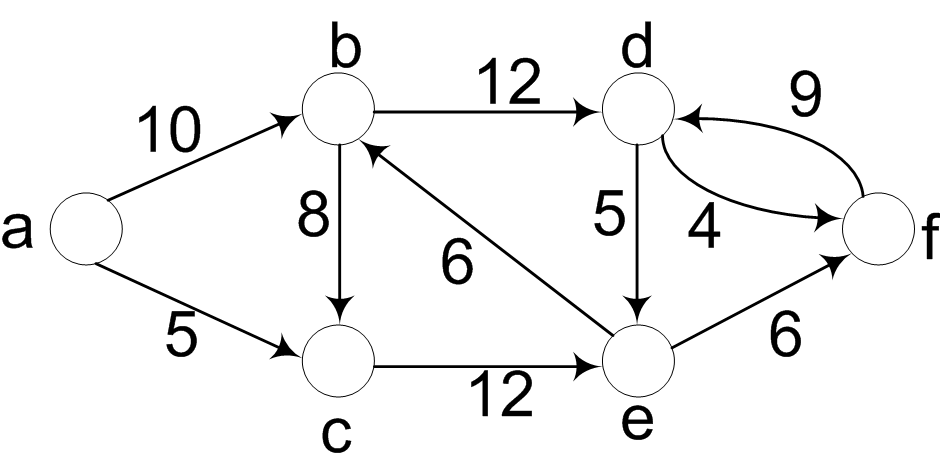
\includegraphics[width=0.5\linewidth]{pics/sp_fig1.png}
	\caption{A directed graph}\label{fig:sp_fig1}
\end{figure}

An example of table is given Table~\ref{tab:example}.
\begin{table}[htb]
	\centering
	\caption{An example of a table}\label{tab:example}
	\begin{tabular}{l|ccccc}
		\toprule
		No of vertices & 64 & 128 & 256 & 384 & 512\\
		\midrule
		Serial &0.1&0.2&0.3&0.4&0.5\\
		Parallel &&&&\\
		Sppedup &2&3&4&5&6\\
		\bottomrule
	\end{tabular}
\end{table} 

\end{document} 

